\documentclass[11pt]{sensys-proc}

\usepackage{graphicx}
\DeclareGraphicsExtensions{.pdf,.jpg,.png}
\graphicspath{{./figs/} {./plots/}}

\usepackage{balance}
\usepackage{comment}
\usepackage{listings}
\usepackage{xspace}
\usepackage[export]{adjustbox}
\usepackage{wrapfig}
\newcommand{\chain}{Chain\xspace}
\numberofauthors{3}

%\author{

% The command \alignauthor (no curly braces needed) should
% precede each author name, affiliation/snail-mail address and
% e-mail address. Additionally, tag each line of
% affiliation/address with \affaddr, and tag the
% e-mail address with \email.

%\alignauthor Amanda Marano \\
%        \affaddr{Department of Electrical and Computer Engineering}\\
%        \affaddr{Carnegie Mellon University}\\
%       \email{amarano@andrew.cmu.edu}
%\alignauthor Emily Ruppel \\
%        \affaddr{Department of Electrical and Computer Engineering}\\
%        \affaddr{Carnegie Mellon University}\\
%       \email{eruppel@andrew.cmu.edu}
%\alignauthor Neil Ryan \\
%        \affaddr{Department of Electrical and Computer Engineering}\\
%        \affaddr{Carnegie Mellon University}\\
%       \email{nryan@andrew.cmu.edu}
%}


\title{TAPIR: Threaded Application Programming on Intermittent Resources}

\begin{document}

\maketitle

%Only including an abstract since it looks like the submission site wants one...
\begin{abstract}
Killer abstract.
\end{abstract}


\section{Introduction/Background}
  \label{sec:intro}
%A/N: I don't think that the paragraphs in this section are in a great order, but I am having a hard time making it flow better.
%Also I'm absolutely sure each of these paragraphs can definitely be bulked up more for length. Please help thank you!!!

The increase in popularity of Internet of Things (IoT) has led to research focus in wireless technologies and low-power computing.
New technologies in both of these areas has led to new
\textit{energy-harvesting computing devices} that operates only with power it has
collected from the surrounding environment \cite{Chain}. These devices have use cases in medical, IoT, and research applications.

Commonly, an energy-harvesting devices charges and collects power in a storage capacitor until the capacitor reaches a sufficient level of charge.
Once the capacitor is charged, the device begins its operation phase and will run until the capacitor is drained.
This leads to the \textit{intermittent execution model} where regular shut downs and reboots to recharge are the common case rather than the rare case in
a traditional execution model. Because the intermittent execution model includes power failures and reboots, continuous execution programs behave
irregular behavior on an intermittent device and a new programming model is needed.

Our multithreaded model is build on two existing programming models, DINO and Chain.
An initial intermittent programming model DINO breaks intermittent programs into tasks, which creates automatic checkpointing locations
during exeuction \cite{Dino}. DINO uses a checkpointing and recovery model that tracks both volatile and nonvolatile memory.
The DINO execution model executes all tasks transactionally, leading to atomic task semantics and does not permit consistency violations in
nonvolatile state \cite{Dino}. Chain, a more recent iteration of the concepts in DINO, uses volatile state rarely, if ever, and uses task boundaries
called channels to store most used data in nonvolatile memory \cite{Chain}. At compile time, Chain allocates the necessary channels between tasks
by parsing channel read and write statements in order to match up aligning tasks. All inputs and outputs to each task, as well as necessary data
structures, are stored in a channel for a respective task. A channel may only be modified by one task, and only one task may run at a time,
which mitigates time of check, time of use bugs (TOCTOU) in intermittence.
The one exception is a self-channel for recursive code, which is double buffered.
Keeping all modifiable data in nonvolatile memory that is not open to easy rewrite makes these tasks idempotent across reboots.
Because of continuous reboots, many operations necessarily will be executed more than once,
and correctness is compromised if those operations are not guaranteed to have the same outcome by the programming model after each reboot.

A main issue in intermittent computing along with idempotence is the Read-Modify-Write (RMW) problem.
Because volatile memory is cleared on each reboot, it is possible that in between reading and modifying or modifying and writing the data had changed,
leading to incorrect answers and an inconsistent state. In the Chain programming model, this problem is solved by creating a new task to house the
problematic operations. Because tasks are blocked by channels that can only be written by one task and are saved to nonvolatile memory, RMW is avoided.
However, in multiprogramming the problem manifests in another way; if the scheduler switches tasks on a reboot, the currently running thread could have
been in the middle of its critical section, making it difficult for other threads to make progress if context switches always occur after a reboot.
Because of this we have decided on a round-robin scheduler with context switches at the end of a task, to guarantee forward progress while knowing
which tasks have run to completion.

In the current Chain programming model, writing code that completes multiple objectives correctly is now difficult.
Current chain programs are small and only have one objective. Additionally, there is no support for advanced control flow.
Multiple control threads may exist, but in the current model there is no support for them and programmability is difficult and often incorrect.
Supporting multiple control threads in Chain also necessitates a linear increase in a limited memory resource, because all large shared data structures
must be copied into each necessary channel, and also makes updating the structures a time consuming, high-overhead task.
In order to increase functionality of chain and to mitigate these shortcomings, we add familiar threading semantics to Chain in order to express
multi-threaded control flow operation. In order to do this we create a lightweight scheduler task that becomes part of the inter-task checkpointing
operation and provide a method of sharing large data structures between tasks with a locking feature. This method is low-memory and low-execution
overhead, which can then maintain the Chain programming semantics at the user level still successfully complete work on an intermittent device.

Example Citation\cite{Chain, Mementos, Aware, Dino}!


%Sample of adding a picture across the top of a split page...

%\begin{figure*}
%\centering
%\begin{minipage}[b]{0.49\textwidth}
%  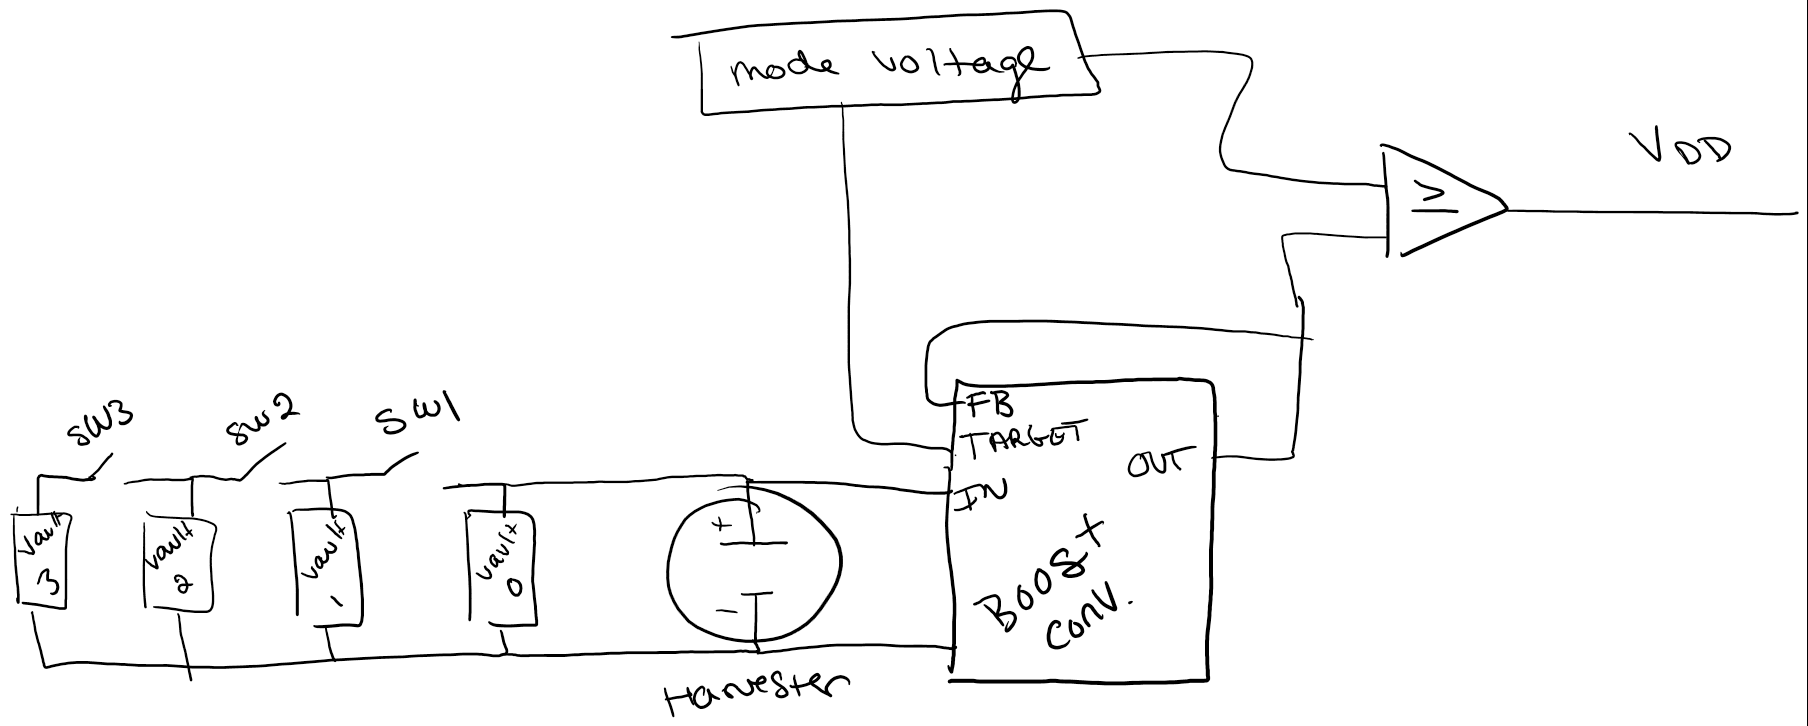
\includegraphics[width=0.95\textwidth,center]{capybara-all.png}
%\caption{Capybara power system overview}\label{label-a}
%\end{minipage}\hfill
%\begin{minipage}[b]{0.49\textwidth}
%  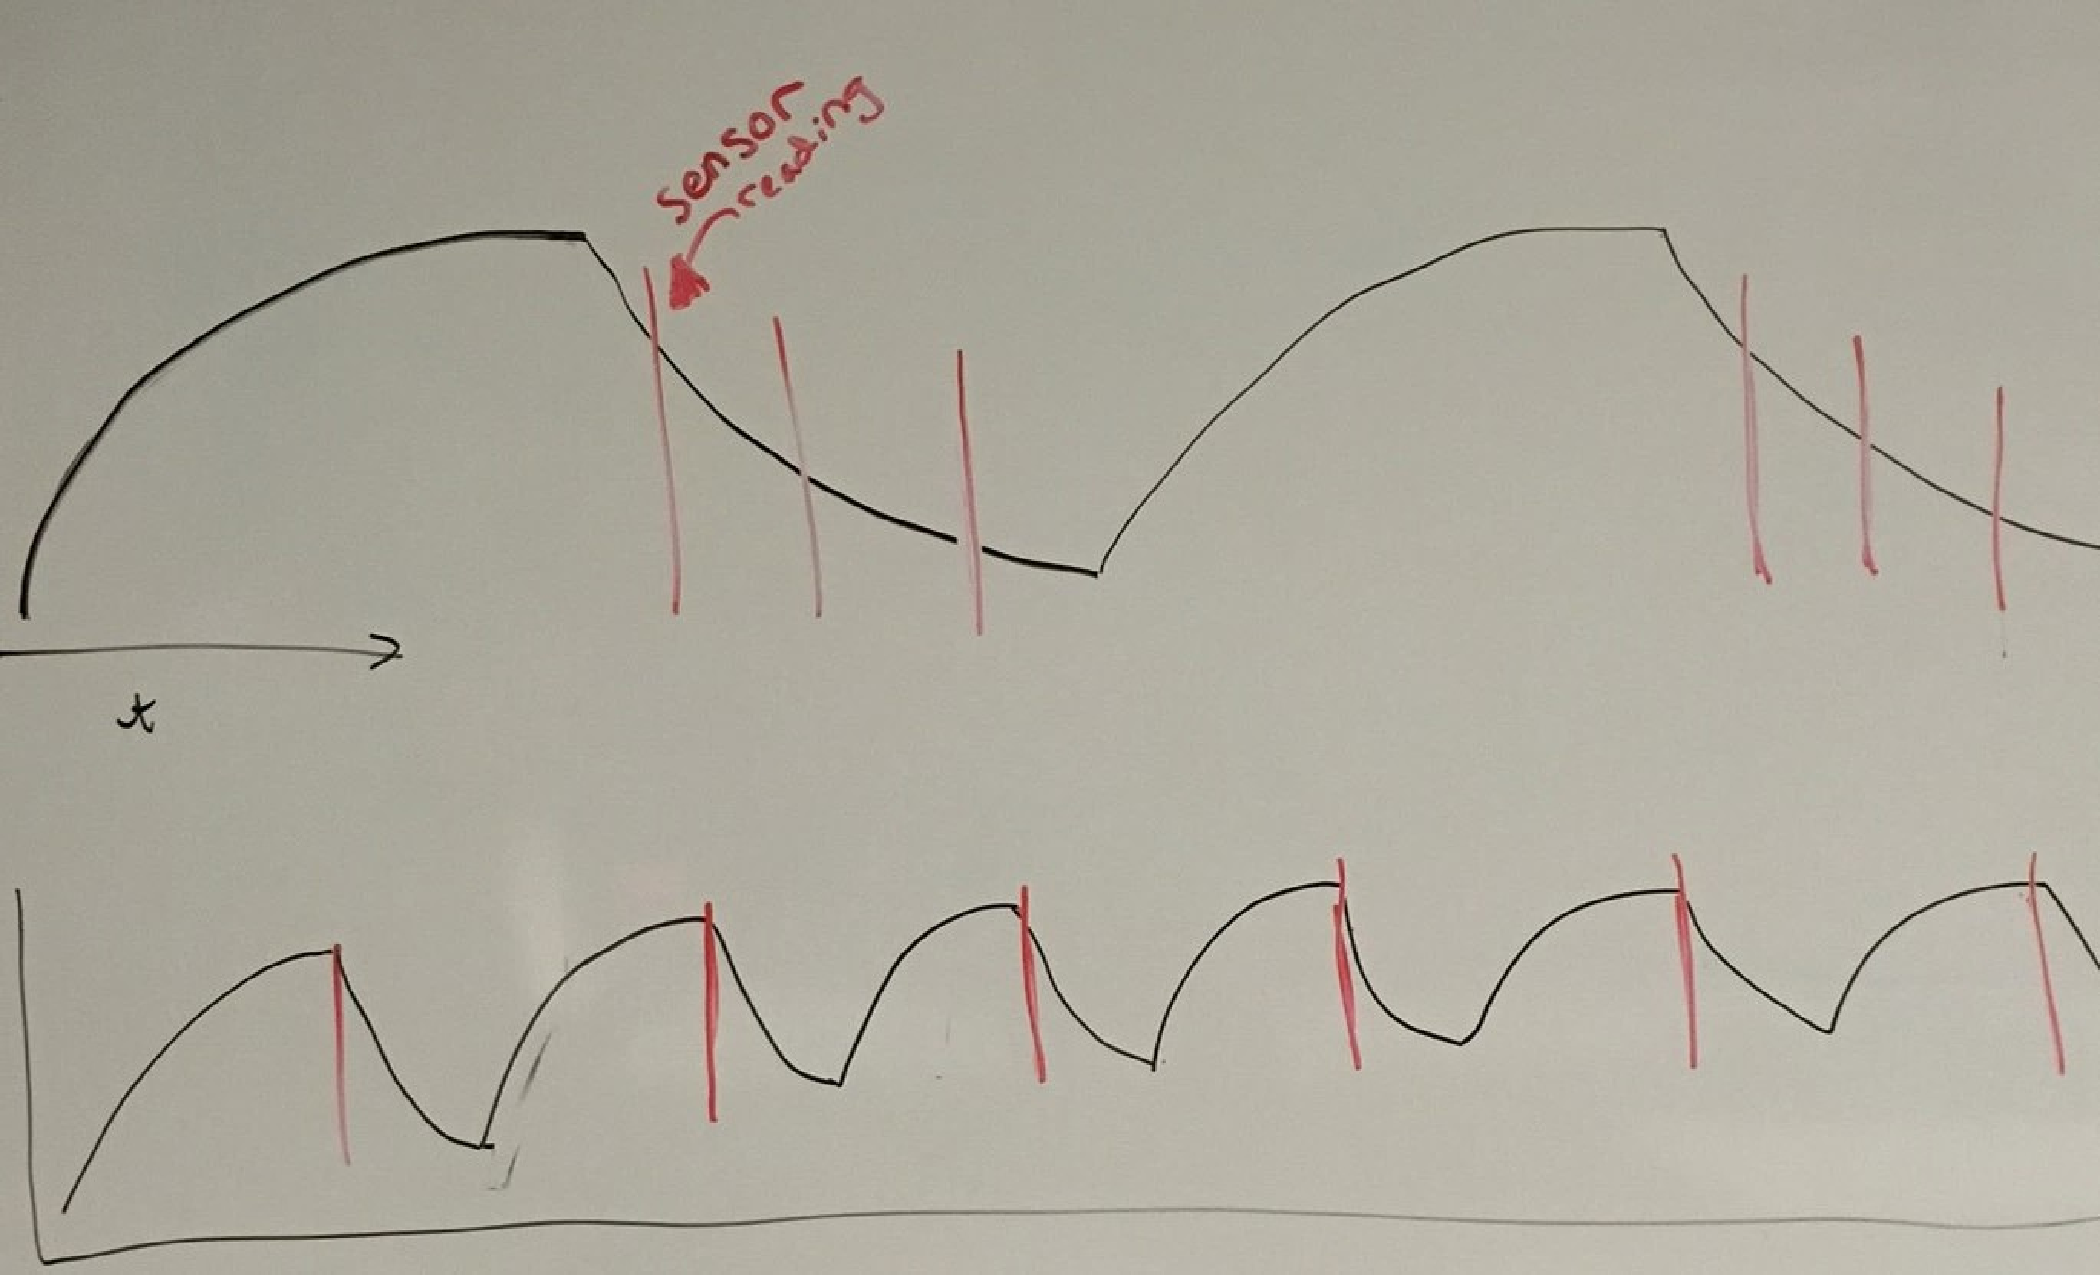
\includegraphics[width=0.95\textwidth,center]{power_modes.pdf}
%\caption{Effect of different power modes}\label{label-b}
%\end{minipage}
%\end{figure*}

More text after the picture to show how that looks...


\section{Related Work} 
In addition to the division of a program into tasks, as described above, prior work
explores several different strategies for preserving state across reboots. The approaches
range from fully independent of the programmer~\cite{ratchet, dewdrop} at one extreme, to programmer
defined task boundaries~\cite{Dino} at the other.  Compiler driven approaches such as the
method used in ~\cite{Mementos} allow the programmer to specify high level behavior of the
checkpointing system. A key similarity among the prior work is it
does not lend itself well to multi-programming let
alone multi-threading. In fact, many of these works state the assumption that the device
hardware cannot support a conventional OS, and thus focus on single threaded programs. 
Despite the availability of (relatively) inexpensive nonvolatile memory technology such as
FRAM~\cite{quickrecall}, the the energy and storage overhead of checkpointing multiple
thread states would limit the maximum per-thread checkpoint size. 

Furthermore, if a multiprogrammed application were implemented using previous
checkpointing strategies, reasoning about thread interleavings becomes  difficult to
reason about because of unpredictable power failures. Any conventional timeout based
thread switching approach will be challenging in an intermittent system, but systems that
allows dynamic checkpointing~\cite{hibernus}, or dynamic task formation~\cite{Dino} become
even more difficult to program. Particularly in systems like ~\cite{Dino} where the
programmer is responsible for placing task boundaries, there is a risk that programmers
will either overuse task boundaries in an effort to preserve any given thread's state, or
underprovision task boundaries such that progress is never made because of context
switching that dynamically expands the number of instructions between task boundaries. 

While prior work has stopped short of suggesting an operating system for intermittently
powered devices, a number of different works touch on the need for these devices to
perform multiple tasks in the same workload. Buettner, Greenstein and Wetherall motivate
their runtime, Dewdrop, based on difference in energy requirements for the tasks that a
CRFID needs to perform~\cite{dewdrop}. The energy aware memory mapping in ~\cite{Aware}
discusses the challenge of handling nondeterministic interrupts received by intermittent
sensing platforms when a peripheral must be serviced immediately and control flow deviates
from single threaded execution. From a hardware standpoint, the federated energy scheme in
~\cite{ufop} provides a platform for removing the energy dependence between an MCU and its
peripherals. Federated energy also simplifies a programmer's reasoning about reading from
a single peripheral. However, federating energy does not help a programmer describe how to
handle {\em multiple} peripherals. Consider a listing in
~\cite{ufop} reporoduced in Figure ~\ref{copy}, and imagine the level of understanding
of the hardware behavior a programmer would have to employ to, say, read one sensor if it
is available but read from and proceed to process data from a different sensor if it is not. 

% Doesn't compile, commenting out
%\begin{figure}[h]
%  \centering
%  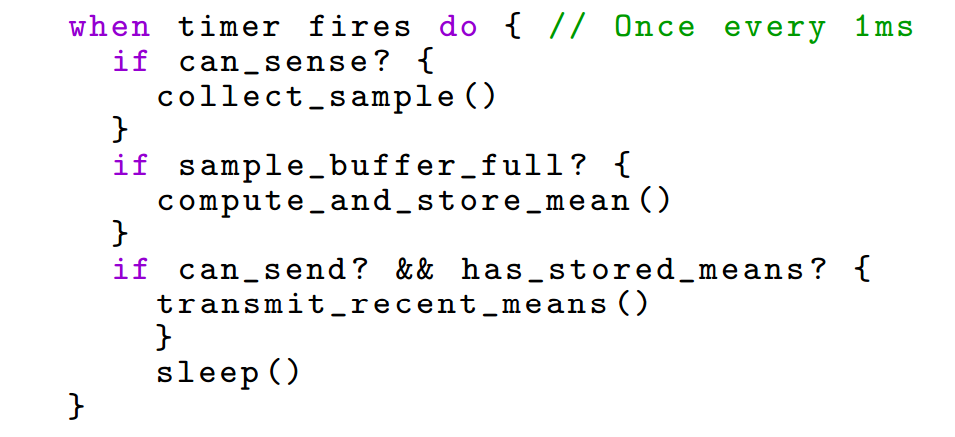
\includegraphics[width=0.99\columnwidth]{figs/listing}
%  \caption{{\bf Example program for sensing and sending data}}
%  \label{fig:copy}
%\end{figure}

The wireless sensor networks community has explored multiple approaches for handling
multitasking on resource limited devices. The designs tend to provide a combination of
timer and event driven context switching as well as a simple programming interface.
TinyOS uses a simple FIFO scheduler to handle event based context switches~\cite{tiny}.
Nano-RK implements priority based preemptive multitasking where task priorities are
statically defined~\cite{nano}. Contiki uses proto-theads, stackless program threads, to
offer a model between nano-RK and tinyOS. The Contiki implements "cooperative
multithreading" such that events can trigger a context switch, but multithreading may also
be timer based~\cite{contiki}. The goal of multitasking interfaces in wireless sensor
networks is to provide a tradeoff between network lifetime and quality of service. This
differs from the intermittent programming model where the challenge is not system
lifetime, but system functionality based on energy availability. 

\section{Chain Discussion}
\chain, while providing a reasonable interface for programmers to work within,
has several inefficiencies that give poor performance on certain applications.
First, there is no notion of data sharing between tasks - all communication is
strictly done through channels. This is useful, as the programmer never needs
to reason about idempotence with respect to their data, but all data that needs
to be transferred between tasks needs to be housed in a channel. Since, under
the original constraints of \chain, channels cannot be written or read from by
tasks that do not own the channel - only tasks that own the channel can access
the data within. This means that large data structures, arrays for instance,
that need to be shared between several channels must be unnecessarily
duplicated in non-volatile memory - one copy of the data structure for each
channel that it needs to be accessed in. Granted, there is no enforcement of
channel ownership by the compiler, but the programmer risks idempotence
violations by straying outside the constraints of chain. We exploit this to
create an equivalent to the multicast-in and multicast-out channels described
in \chain, but using them requires much more reasoning on the part of the programmer.


Additionally, since dynamic memory allocation is arguably too expensive to run
on intermittently powered systems, memory is allocated at compile time.
Unfortunately, since there isn't a compiler specifically for \chain, arrays
are statically sized based on \texttt{\#define} parameters. This can be
create tricky memory corruption errors for the programmer when out-of-bounds
array accesses occur because, for instance, a self-channel has more dirty
fields than \texttt{MAX\_NUM\_DIRTY\_FIELDS}.


\chain also struggles with long-range control flow. For each transition to a
new task, the transition is an explicit one-to-one mapping. \chain provides no
semantics, for instance, to transfer control from task A to task B, then also
transfer control to task C after task B completes, without the programmer
placing \texttt{TRANSITION\_TO(task\_C)} inside task B. This could be done by
using channels in a similar manner to function pointers, while staying within
the semantics of \chain (as we did), but reasoning about code becomes more
challenging for the programmer.


Future work for \chain needs to include some sort of memory allocation based on
the set of channels allocated in the program, but this is work for a compiler
and beyond the scope of this work. For our purposes of threaded applications,
however, \chain is a sufficient launching pad, despite its misgivings since it
does not require specialized hardware or energy subsystems to work effectively,
and since it solves the issue of idempotent data accesses in a way that is
abstracted from the programmer.


\section{What we did} % TODO change title
Mutexes - Emily\\
Round Robin (alternatives, on reboot)\\
SIMD vs MIMD\\
SIMD w/ channels (you don't get your own registers...etc -
    just channels, since intermittent)\\


\subsection{Scheduler}
For a multi-threaded programming model to exist, one must create a structure to
switch between multiple threads. To keep with \chain's model, we chose to make
the scheduler its own task. The alternative is possible, but since our
implementation of the scheduler required multicast channels, it makes more
sense to have the multicast channels have one endpoint well defined, instead of
some sort of all-to-all channel (which is just a global location in
non-volatile memory). The multicast channels channels are not strictly
necessary, but, all in all, we believe that keeping the scheduler as an
explicit task is good for abstraction. Additionally, if a task has few
self-channels and the data structures passed in those self-channels are
relatively small, the overhead of transitioning to that task is relatively
small, as few double-buffers for self-channels need to be flipped (which is
arguably the largest overhead).


\subsection{Programming Model}
Threaded applications that use POSIX or some other standard library interface
tend to use function calls to interact with the library - for instance, the
user calls a function \texttt{thread\_create} to spawn off a thread.
Unfortunately, this is a difficult programming model to keep under
intermittence, since function calls like \texttt{thread\_create} tend to
involve non-idempotent actions, like appending to a list or incrementing a
variable's value. This leaves two clear options - making the functions to
interact with our threading library \chain tasks, or adding infrastructure to
to our threading library to make the non-idempotent actions that need to occur
act idempotently. We opted for the latter - we feel that it is more valuable to
maintain programmability by provide the user with an interface that they
expect, instead of trying to extend a \chain semantic like
\texttt{TRANSITION\_TO} to also include thread creation.


\subsection{Interrupts}
\subsubsection{Motivation}
Ideally, multithreading would extend to a programming model that can utilize
interrupts in a producer/consumer fashion (i.e. a thread is waiting on data
from an external source, the external source fires an interrupt, the thread
samples the external source and stores the received data in a buffer, and
the thread returns to its original task). However, the inherent
non-deterministic
nature of interrupts from, say, an ADC, creates additional complexity for the
programmer when reasoning about shared memory, especially with respect to
idempotence.


    Specific to the MSP430 architecture (but common in other systems), there is
also the issue of stack integrity. On the MSP430, when an interrupt fires,
the program counter and status register are pushed onto the stack for
the handler to be able to return back to the state of the machine when the
interrupt fired. In our case, however, where power failure is the common
case, an application could experience failure while inside an interrupt
handler. This raises two issues. First, upon reboot from a power failure,
the stack will be cleared (since the stack is stored in volatile memory) and
execution will return to the handler, if we assume that the interrupt handler
is a \chain task. Upon leaving the interrupt, via the MSP430 RETI instruction),
the program's behavior will be undefined. Second, if the programmer does not
use a \chain task for the interrupt handler, it is possible that the interrupt
could fire when the system has a low amount of energy remaining, thus
rendering the system unable to finish executing the interrupt handler,
leading to a host of potential problems.


\subsubsection{Interface}
We provide the functions and macros in figure 3 as an interface to
the programmer. The standard workflow is as follows: the programmer
designates the task that should be run on an interrupt firing
with \texttt{INTERRUPT\_TASK(val, func)} where \texttt{val} is the task
index and \texttt{func} is the function that will be called upon an
interrupt firing - \texttt{val} and \texttt{func} follow the same
interface as \chain tasks. Since we assume that the handler is not
reentrant, the programmer replaces calls to \texttt{\_\_enable\_interrupt()}
with our function \texttt{enable\_interrupts()}.
The programmer's code remains unmodified, with the exception of a call to
\texttt{int\_setup\_complete()} when the \chain program has finished whatever
register initialization is necessary to setup the interrupts for the
application.\\


\begin{figure*}
\begin{minipage}[b]{1.0\textwidth}
\begin{lstlisting}
    /** Enable interrupts if int_setup_complete() has been called
      * and execution is not inside an interrupt handler */
    void enable_interrupts();

    /** To be called when setup for the interrupt handler is complete,
      * also enables interrupts */
    void int_setup_complete();

    /** Return from the interrupt handler */
    void return_from_interrupt();

    /** Designate a task to run when an interrupt fires */
    INTERRUPT_TASK(val, func)
\end{lstlisting}
\caption{Interrupt Handling Interface}\label{label-a}
\end{minipage}\hfill
\end{figure*}

\subsubsection{Design}
Working within the constraints of \chain and our multi-programming extensions,
we work to provide a layer of abstraction to the programmer through the standard
layer of tasks and channels. Notably, this includes interrupt handlers being
tasks, rather than standard functions. The alternative has been explored
by keeping specific capacitors for interrupt handlers\cite{Aware}, but this
approach fails if interrupt handlers take longer than the capacitor has
energy for. This bug handlers not completing due to power failure is
unintuitive for programmers coming from consistently powered devices and
makes certain devices unusable under intermittent power.


With interrupt handlers as tasks, if a power failure occurs during a
handler, execution will resume at the handler. This isn't ideal, the
standard paradigm that interrupt handlers are generally short and fast
so that interrupts won't be missed (for instance, a timer interrupt
being missed because processing the interrupt took longer than the
timer period), but we argue that it is more unreasonable to say
that interrupt handlers that take too long will not complete than
to violate the standard paradigm, since the former arbitrarily restricts
the application domain.


For the sake of simplicity, we assume that interrupt handlers are not
reentrant. Since reentrant handlers can be used in a non-reentrant fashion
without consequences, this assumption does not restrict the application domain.
Moreover, the benefit to reentrant handlers, the application will not miss an
interrupt firing because processing the previous one took too long, is
secondary on intermittent architectures - there is likely a higher chance that
a power failure will occur than an interrupt handler causing an interrupt to be
missed, unless interrupts are firing on an extremely fine granularity.


When an interrupt handler has completed, the programmer calls
\texttt{return\_from\_interrupt()}, which returns execution to the start
of the task that was running when the interrupt occurred. This contradicts
expected behavior - on continuously powered systems, execution generally
returns to the instruction after the instruction that the system received an
interrupt while processing. The continuous system model is intuitive, but
breaks under \chain's intermittence. Task idempotence in \chain only works
when execution returns to the top of a
task upon power failure. Program state (registers and stack memory) are stored
in volatile memory, if an interrupt handler returned to the middle of a task,
it would be impossible to reason about program correctness, since none of the
program state had been stored. The programmer could store program state on the
stack at the start of interrupt handlers, but this would be lost on power
failure. She could also store this program state in non-volatile memory -
trivial for the register set, but difficult and potentially extremely costly to
store the stack, as execution could be several functions deep. Even determining
how much stack to save could be prohibitively costly. Another alternative would
be to store program state in non-volatile, but this has been shown to be
prohibitively costly in most applications \cite{Aware}.


\section{Implementation}
Scheduler Data structures and idempotence (what we broke and why) -NEIL\\
Mutexes (Simple, meant for pseudo channels) - Emily\\
Interrupts (mucked with IE flags) - Neil\\
% Interrupt prologue
% Interrupt setup


\section{Results} - Emily
No really, there will be things here!
Applications/measurements\\
Blinker (x2)\\
RSA+cukoo\\
No verification\\
Memory overhead (read off compilation)\\
Performance (\# reboots)\\


\section{Future Work}
Future work is focused on saving memory by using channel and code reuse optimizations when forking new chain programs from current tasks.
When forking a new task, a channel may be duplicated, which linearly increases the amount of memory necessary for channels with the number of currently running programs.
It is possible to reuse channels between tasks if the number of iterations of that task are known at compile time and it can be estimated how
many are to be running simultaneously. A register allocation graph coloring scheme can then be repurposed for reusing channels allocated at compile time.
In either case the current channel naming scheme must be changed to support channel duplication, ether real or simulated.
Currently channels are allocated and named at compile time by combining the names of the input and output channel tasks.
However, if tasks can be duplicated this naming scheme must be altered to support multiple channels of the same name and potentially multiple channels of the same name.
This can be done with a vector clock timestamp or a simple counter stored in nonvolatile memory to create unique channel names.

Additionally, it is possible to save memory by sharing arrays between tasks without the necessity of copying the array in its entirety in each channel.
To do this the concept of intermittent tasks mutexes for shared resources and data structures would be introduced.
The structures are protected by a lock that contains the thread ID of the task that currently holds the lock.
In order to allow all tasks access to a data structure without breaking all chain semantics, a modified version of a module channel would be used in order
for multiple tasks to potentially modify one channel.
However, even with that change it is challenging to define sharing between threads in an intermittent context and to maintain chain semantics while implementing
shared data structures while still maintaining correctness.
Because channel sizes are constrained at compile time currently, it is also necessary to know at compile time all data structures, shared or private,
that are going to be used during execution of a chain program or programs.
It is a challenge for future work in this field to constrain memory for channels at compile time and for the compiler to know with certainty how much memory
is necessary to allocate. Depending on the workload, the amount of forked threads would need to be constrained such that threads don't overflow nonvolatile memory at runtime.

Future work also includes optimizations to reduce overhead, such as converting the free indices array to a free indices bitmap in order to reduce the amount of
baseline memory that the scheduler task uses.
Re-assignation and re-use of channels at runtime would increase overhead, but it is thought that the memory saved by this procedure is worth the trade-off of increased overhead.
If re-assignation can be determined at compile-time, the overhead during runtime will still remain low.

\section{Conclusion}
Multithreading in intermittence {\em is} a good idea!

% Doesn't compile, commenting out
%\begin{figure}[ht]
%  \centering
%  
\includegraphics[width=0.9\columnwidth]{figs/tapir}
%\end{figure}


\balance
\bibliographystyle{abbrv}
\bibliography{sigproc}  % sigproc.bib is the name of the Bibliography
\end{document}
